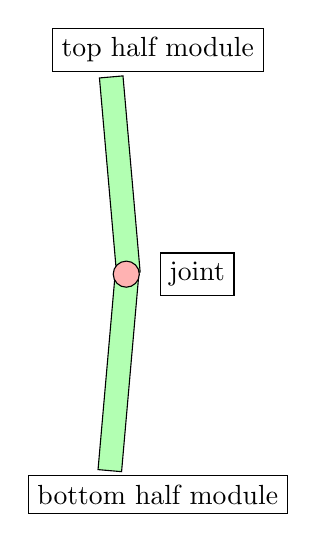
\begin{tikzpicture}
    \node[rectangle, 
    draw = black, 
    fill = green!30!white, 
    minimum width = 0.3cm, 
    minimum height = 2.5cm,
    rotate around = {-5:(0,0)}] at (0,0) {};
    \node[rectangle, 
    draw = black, 
    fill = green!30!white, 
    minimum width = 0.3cm, 
    minimum height = 2.5cm,
    rotate around = {5:(0,2.5)}] at (-0.2,2.5) {};
    \node[circle, 
    draw = black, 
    fill = red!30!white, 
    minimum width = 0.01cm] at (0.1,1.25) {};

    \node[draw, align=left] at (0.5, 4.1) {top half module};
    \node[draw, align=left] at (1, 1.25) {joint};
    \node[draw, align=left] at (0.5, -1.55) {bottom half module};
\end{tikzpicture}